\newpage
\section{Timeline}
During this project there are many smaller, that is not to say lesser, subject that needs to be touched upon. All of the areas that need investigation has some sort of dependencies which means that work needs to be carried out in some order. To this end we have approximately mapped out these dependencies, and arranged them in what seems a logical arrangement as showed in the preliminary fig \ref{fig:dependency_graph} on page \pageref{fig:dependency_graph}.   

Except each project members daily commitment to this project we have 4 weekly meetings as show in table \ref{tab:schedule} on page \pageref{tab:schedule}, aside from these, members will teem up iteratively on different subjects and share larger workloads.  

Initially the work will be skewed to researching and self study but later to report writing...

\begin{table}[]
\centering
\begin{tabular}{llll}
\hline
Day & Location & Time  & Kind            \\ \hline
Mon & Digital  & 11.00 & Weekly Planning \\
Tue & Chalmers & 10.00 & General         \\
Tue & Chalmers & 11.00 & Supervisor      \\
Fri & Digital  & 13.00 & Weekly Checkup 
\end{tabular}
\caption{Schedule}
\label{tab:schedule}
\end{table}


\begin{figure}
  \makebox[\textwidth][c]{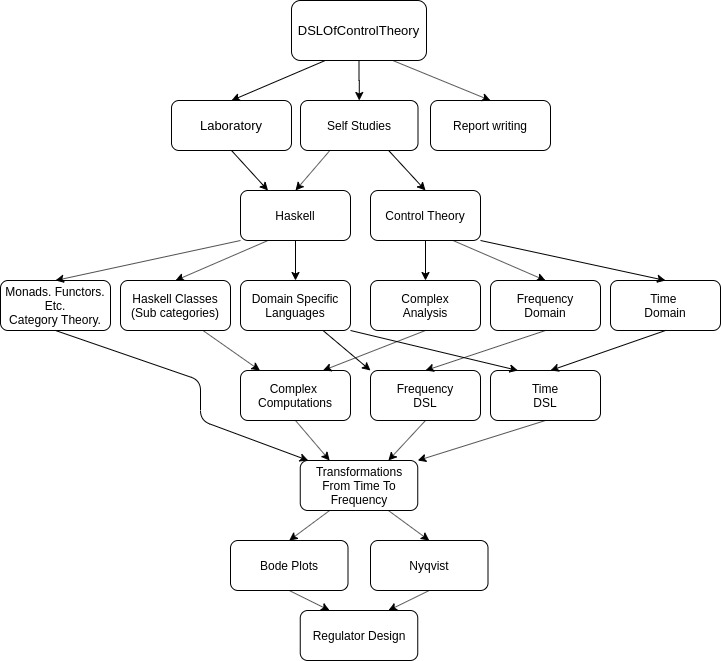
\includegraphics[width=1.4\textwidth]{DependencyGraph.jpg}}%
  \caption{Possible dependency graph.}
  \label{fig:dependency_graph}
\end{figure}




\iffalse
Tidsplan
Beskriver vad som ska göras och när det ska göras

Planera aktiviteter i detalj för den närmaste tiden, grovt för senare delar – uppdatera after hand

Att jobba iterativt och successivt uppdatera planen och rapporten är ofta effektivt 

Var konkret – då kan handledare och andra berörda ge bra synpunkter och planen kan bättre vägleda arbetet
\fi